\chapter{FUNDAMENTAÇÃO TEÓRICA}\label{cap:cap2}

\section{SÉRIES DE TAYLOR}
A expansão em séries de Taylor é uma ferramenta importante na matemática que permite aproximar uma função 
$f(x)$
desconhecida ou complicada por meio de um polinômio. Para isso, ela deve ser suficientemente suave, contínua e diferenciável \cite{Guidorizzi}.
A série é construída a partir das derivadas da função em um ponto específico 
$x_0$
, chamado ponto de expansão.

A forma geral é dada pela equação \eqref{eq:taylor_geral}:
\begin{equation}\label{eq:taylor_geral}
    f(x) = f(x_0) + f'(x_0)(x-x_0) + \frac{1}{2!}f''(x_0)(x-x_0)^2 +\dotsb+ \frac{1}{n!}f^{n}(x_0)(x-x_0)^n + \dotsb
\end{equation}

Vale ressaltar que a expansão se aproxima cada vez mais da função original conforme a série é truncada com um maior número de termos \cite{atkinson1989introduction}.
Pode-se, ainda, usar o teorema do erro de Taylor e ter uma estimativa do erro entre a função original em um ponto $b$,  e sua aproximação polinomial truncada no termo $n$ e avaliada em um ponto de expansão $x_0$, conforme a equação \eqref{taylor_erro}.
\begin{equation}\label{taylor_erro}
    E(b) = \frac{f^{n+1}(b)}{(n+1)!}(x-x_0)^{n+1}
\end{equation}

Para uma função multivariada $f(X)$ em que $X= [x_1,x_2,\cdots,x_k]^T$
, a expansão de Taylor até a segunda ordem é dada por \eqref{eq:taylor_multivariavel}.
\begin{equation}\label{eq:taylor_multivariavel}
f(X) \approx  f(X_0) + \nabla f(X_0).(X-X_0) + \frac{1}{2!} (X-X_0) H(X_0) (X-X_0)^T
\end{equation}

Onde o gradiente de $f$ avaliado em $X_0$ é dado por \eqref{eq:gradiente}.
\begin{equation}\label{eq:gradiente}
    \nabla f(X_0) = 
    \left.
    \begin{bmatrix}
        \frac{\partial f}{\partial x_1} \\
        \vdots \\
        \frac{\partial f}{\partial x_k}
    \end{bmatrix}
    \right|_{\substack X = X_0}
\end{equation}

E a matriz Hessiana $H$ avaliada em $X_0$ é obtida através de \eqref{eq:hessian_matrix}.
\begin{equation}\label{eq:hessian_matrix}
    H(X_0) = 
    \left.
\begin{bmatrix}
\frac{\partial^2 f}{\partial x_1^2} & \frac{\partial^2 f}{\partial x_1 \partial x_2} & \cdots & \frac{\partial^2 f}{\partial x_1 \partial x_k} \\
\frac{\partial^2 f}{\partial x_2 \partial x_1} & \frac{\partial^2 f}{\partial x_2^2} & \cdots & \frac{\partial^2 f}{\partial x_2 \partial x_k} \\
\vdots & \vdots & \ddots \\
\frac{\partial^2 f}{\partial x_k \partial x_1} & \frac{\partial^2 f}{\partial x_k \partial x_2} & \cdots & \frac{\partial^2 f}{\partial x_k^2} \\
\end{bmatrix} 
\right|_{\substack X = X_0}
\end{equation}

De acordo com Tinney et al. (\citeyear{NewtonRaphson}), o método de Newton-Raphson pode ser aplicado para encontrar raízes de sistemas de equações não lineares
$F(X) = [f_1(X), f_2(X),\cdots,f_k(X)]^T$, que é o caso do problema do \acs{FP}.

A forma geral, truncada na segunda ordem, é apresentada pela equação \eqref{eq:sistema_multi_taylor}:
\begin{equation}\label{eq:sistema_multi_taylor}
    F(X) \approx F(X_0) + J(X_0)(X-X_0) + \frac{1}{2!}(X-X_0)^T H(X_0)(X-X_0)
\end{equation}

Onde $J(X_0)$ é a matriz Jacobiana avaliada em $X_0$, dada por \eqref{eq:Jacobiana_multi}:
\begin{equation}\label{eq:Jacobiana_multi}
    J(X_0)= 
    \left. 
    \begin{bmatrix}
    \frac{\partial f_1}{\partial x_1} & \cdots & \frac{\partial f_1}{\partial x_k} \\
    \vdots & \ddots & \vdots \\
    \frac{\partial f_k}{\partial x_1} & \cdots & \frac{\partial f_k}{\partial x_k} 
    \end{bmatrix}
    \right|_{\substack{X = X_0}}
\end{equation}

E $H(X_0)$ é o tensor Hessiano avaliado em $X_0$, dado por \eqref{eq:Hessian_tensor}:

\begin{equation}\label{eq:Hessian_tensor}
    H(X_0) = 
    \left. 
    \begin{bmatrix}
        \begin{bmatrix}
            \frac{\partial^2 f_1}{\partial x_1^2} & \frac{\partial^2 f_1}{\partial x_1 \partial x_2} & \cdots & \frac{\partial^2 f_1}{\partial x_1 \partial x_k} \\
            \frac{\partial^2 f_1}{\partial x_2 \partial x_1} & \frac{\partial^2 f_1}{\partial x_2^2} & \cdots & \frac{\partial^2 f_1}{\partial x_2 \partial x_k} \\
            \vdots & \vdots & \ddots \\
            \frac{\partial^2 f_1}{\partial x_k \partial x_1} & \frac{\partial^2 f_1}{\partial x_k \partial x_2} & \cdots & \frac{\partial^2 f_1}{\partial x_k^2} 
        \end{bmatrix}
        \\
        \\
        \begin{bmatrix}
            \frac{\partial^2 f_2}{\partial x_1^2} & \frac{\partial^2 f_2}{\partial x_1 \partial x_2} & \cdots & \frac{\partial^2 f_2}{\partial x_1 \partial x_k} \\
            \frac{\partial^2 f_2}{\partial x_2 \partial x_1} & \frac{\partial^2 f_2}{\partial x_2^2} & \cdots & \frac{\partial^2 f_2}{\partial x_2 \partial x_k} \\
            \vdots & \vdots & \ddots \\
            \frac{\partial^2 f_2}{\partial x_k \partial x_1} & \frac{\partial^2 f_2}{\partial x_k \partial x_2} & \cdots & \frac{\partial^2 f_2}{\partial x_k^2} 
        \end{bmatrix}
        \\
        \vdots
        \\
        \begin{bmatrix}
            \frac{\partial^2 f_k}{\partial x_1^2} & \frac{\partial^2 f_k}{\partial x_1 \partial x_2} & \cdots & \frac{\partial^2 f_k}{\partial x_1 \partial x_k} \\
            \frac{\partial^2 f_k}{\partial x_2 \partial x_1} & \frac{\partial^2 f_k}{\partial x_2^2} & \cdots & \frac{\partial^2 f_k}{\partial x_2 \partial x_k} \\
            \vdots & \vdots & \ddots \\
            \frac{\partial^2 f_k}{\partial x_k \partial x_1} & \frac{\partial^2 f_k}{\partial x_k \partial x_2} & \cdots & \frac{\partial^2 f_k}{\partial x_k^2}    
        \end{bmatrix}
    \end{bmatrix}
    \right|_{\substack{X = X_0}}
\end{equation}

\section{MÉTODO DE NEWTON RAPHSON}
Muitos sistemas físicos complexos são descritos por equações as quais não possuem uma solução analítica direta, por isso técnicas para obter uma solução numérica aproximada foram desenvolvidas \cite{Stagg}.
Desenvolvido no século XVII por Isaac Newton e Joseph Raphson, o método de Newton-Raphson (\acs{NR}) é um algoritmo que permite encontrar raízes de uma função desconhecida,  desde que se tenha acesso ao valor da função e sua derivada em diferentes pontos. 

Nessa seção, será apresentada a fundamentação teórica do método.
\subsection{Formulação}
O método de NR começa definindo-se uma aproximação inicial
$X_0$
para as raízes procuradas e utilizando essa aproximação como ponto de expansão da série de Taylor, que será truncada na primeira derivada, apresentado abaixo por \eqref{eq:taylor_NR_1}:

\begin{equation}\label{eq:taylor_NR_1}
    F(X) \approx F(X_0) + J(X_0)(X-X_0)
\end{equation}

Ou, por \eqref{eq:taylor_jacobiana}:
\begin{equation}\label{eq:taylor_jacobiana}
    F(X) \approx F(X_0) + J(X_0)\Delta X
\end{equation}

Onde, $\Delta X$ é chamado de incremento de $X$ e é dado por \eqref{eq:deltax}:

\begin{equation}\label{eq:deltax}
    \Delta X = X-X_0
\end{equation}

Como se deseja encontrar as raízes do sistema de equações 
$F(X)$
, iguala-se o lado esquerdo da equação \eqref{eq:taylor_jacobiana} a zero, obtendo-se o valor do incremento 
$\Delta X$, que será usado como ponto de expansão da série de Taylor da próxima iteração $n+1$, como mostram as equações \eqref{delta_x_2} \eqref{eq:atualização_x_0} e \eqref{eq:n=n+1}.

\begin{equation}\label{delta_x_2}
    \Delta X^{(n)} = [J(X_0^{(n)})]^{-1}.\,F(X_0^{(n)})
\end{equation}   

\begin{equation}\label{eq:atualização_x_0}
    X_0^{(n+1)} = X_0^{(n)} + \Delta X^{(n)}
\end{equation}

\begin{equation}\label{eq:n=n+1}
    n = n+1
\end{equation}

Novamente é calculado o valor de $F(X_0^{(n)})$ e avaliado se obedece um erro máximo aceitável
$\epsilon$. Se o erro for maior, mais uma iteração será feita e o processo se repete. Existem casos que o método não consegue encontrar raízes que obedeçam ao erro, por isso define-se um número máximo de iterações $n_{max}$ suficientemente grande para que, caso seja extrapolado, diz-se que o processo divergiu.

Na figura \ref{fig:diagrama_NR}, um fluxograma representativo do método de Newton-Raphson é apresentado, sendo dividido em blocos para sua explicação em detalhes:

\begin{itemize}
    \item Bloco 1: Início do método de Newton-Raphson;
    \item Bloco 2: Inicializa as variáveis de iterações $n$, do incremento $\Delta X$ e da estimativa inicial para as variáveis de estado $X_0$;
    \item Bloco 3: Calcula o valor da função no ponto de expansão $X_0$;
    \item Bloco 4: Avalia se o valor da função com a estimativa atual é menor ou maior ou igual que o erro máximo aceitável $\epsilon$;
    \item Bloco 5: Caso o valor da função não respeite $\epsilon$, atualiza-se o contador de iterações $n$;
    \item Bloco 6: Avalia se o contador de iterações extrapolou o número máximo de iterações $n_{max}$;
    \item Bloco 7: Calcula a Jacobiana avaliada em $X_0^{n-1}$;
    \item Bloco 8: Com a Jacobiana, calcula o incremento $\Delta X^{n-1}$;
    \item Bloco 9: Atualiza $X_0$ na iteração $n$ com o incremento calculado;
    \item Bloco 10: Caso o valor da função respeite $\epsilon$, o processo finaliza com convergência;
    \item Bloco 11: Caso o número de iterações extrapole o $n_{max}$, o processo se encerra sem uma raíz com erro máximo desejado, indicando divergência.
\end{itemize}

\begin{figure} [H]
    \centering
    \caption{Fluxograma do método Newton-Raphson}
    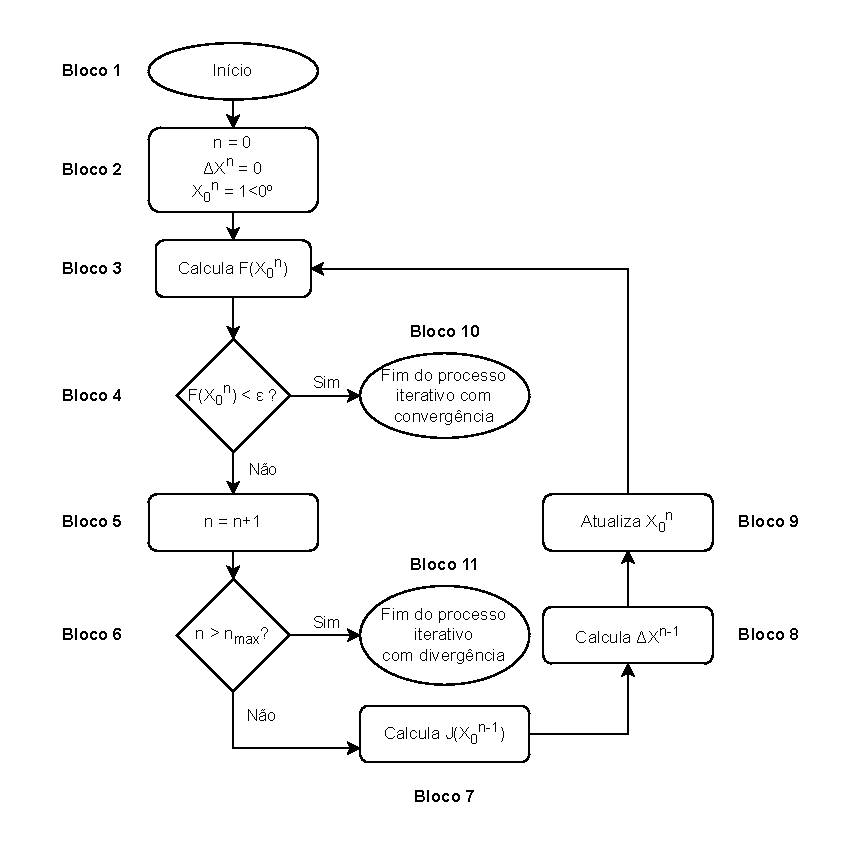
\includegraphics{textuais/capitulo2/figuras/Diagrama_NR_4.drawio.pdf}
    \caption*{Fonte: Elaborada pelo autor}
    \label{fig:diagrama_NR}
\end{figure}


\subsection{Características importantes do método}
O método de NR é altamente dependente do palpite inicial para o vetor de variáveis de estado $X$. Isso ocorre porque a série de Taylor truncada no primeiro termo só se comporta bem em regiões muito próximas da solução. 

Se 
$X_0$
for de fato próximo da solução, a diferença entre a solução atual e a solução verdadeira diminui quadraticamente a cada iteração, característica do método de Newton-Raphson \cite{NewtonRaphson}.

Porém, se 
$X_0$
for um valor muito distante da solução, o sistema pode divergir, levando a nenhuma solução ou a soluções sem sentido físico (soluções instáveis ou espúrias), mesmo que haja uma solução possível para o sistema.

Além disso, pode ser que o sistema de fato não possua solução. Isso também pode ser um problema, principalmente para estudos de planejamento da expansão de um sistema elétrico de grande porte.
Dependendo do caso, é necessário obter uma estimativa da solução, visando entender quais melhorias o sistema precisa para alcançar a convergência na região viável.

Finalmente, é possível que o método não encontre solução quando a matriz Jacobiana é singular ou muito próxima da singularidade. Nesses casos, a inversão de $J$ se torna indefinida, impedindo obter soluções para o problema.

Para combater esse problema de convergência, diversos métodos foram propostos na literatura como o Fluxo de Potência Continuado e outros métodos de otimização heurísticos, como Algoritmos Genéticos.

Um desses métodos é o método do Multiplicador Ótimo, que será visto aprofundadamente no Capítulo \ref{cap:cap3}.

\section{FLUXO DE POTÊNCIA USANDO NR}
O Fluxo de Potência é um procedimento essencial na análise de sistemas elétricos de potência, pois visa determinar o estado operativo da rede elétrica em regime permanente \cite{ONSsubmodulo2_3}. 

Em outras palavras, considerando as características das cargas a serem conectadas, os tipos de geradores, os limites de geração e os limites operativos das linhas, o objetivo principal é determinar:
\begin{itemize}
    \item Tensões nodais: magnitudes e ângulos das tensões em todas as barras (ou nós) do sistema;
    \item Potência reativa dos geradores;
    \item Fluxo de potência nas linhas: Avaliar se as linhas estão operando próximas de seus limites.
\end{itemize}

Nesta seção, será abordado como representar uma rede elétrica, os tipos de barras, as equações de potência e, finalmente, como utilizar o método NR para o problema.


\subsection{Matriz admitância nodal}
A matriz admitância nodal, ou matriz 
$Y_{barra}$
, desempenha um papel fundamental na análise de circuitos elétricos de potência, sendo uma representação matricial dos parâmetros do circuito. Sua importância reside no fato de que ela permite relacionar o vetor
$\Dot I$
de correntes injetadas nos nós
com o vetor
$\Dot V$
de tensões nodais do sistema, de acordo com \eqref{eq:I=YV}. Vale ressaltar que a formulação apresentada é válida apenas para representações monofásicas e sem mútuas \cite{Robba}.

É uma matriz quadrada e simétrica de ordem
$n \times n$
, em que 
$n$
é o número de nós do sistema.
\begin{equation} \label{eq:I=YV}
    \Dot I = Y \, \Dot V
\end{equation}

Uma vantagem de seu uso é que sua formação é simples e pode ser feita por inspeção visual do sistema:
\begin{itemize}
    \item Elementos diagonais “$Y_{kk}$”: Soma de todas as admitâncias conectadas ao nó "$k$";
    \item Elementos não diagonais "$Y_{km}$": Negativo da admitância equivalente entre o nó "$k$" e o nó "$m$".
\end{itemize}

Como o número de nós conectados a um nó específico é limitado em um \ac{SEP}, a 
${Y_{barra}}$
se torna uma matriz esparsa, aumentando seu grau de esparsidade quadraticamente conforme o número de barras aumenta em um sistema. Formas de lidar com essas matrizes computacionalmente, evitando armazenar muitos zeros já são uma realidade nos programas de \ac{FP} atuais, mas não serão tratados neste trabalho.

\subsection{Equações Algébricas do Fluxo de Potência}

As equações algébricas do \ac{FP} apresentadas são conhecidas na literatura por formulação por injeção de potência.
Baseado nas leis de Kirchoff, as potências ativas e reativas injetadas em uma barra $k$ podem ser determinadas através das equações \eqref{eq:PkQk_esp}, onde em termos práticos, a potência gerada $P_{gerada, k}$ e $Q_{gerada, k}$ é a potência fornecida por geradores conectados a barra $k$ e a potência demandada $P_{demandada, k}$ e $Q_{demandada, k}$ é a potência consumida por cargas conectadas a barra $k$.
\begin{equation} \label{eq:PkQk_esp}
    \begin{split}
        P_k &= P_{gerada,k} - P_{demandada,k} \\
        Q_k &= Q_{gerada,k} - Q_{demandada,k} 
    \end{split}
\end{equation}

Logo, a potência complexa injetada em uma barra $k$ pode ser definida em \eqref{eq:S_k} através das tensões e correntes nodais:
\begin{equation} \label{eq:S_k}
     S_k = P_k + j\,Q_k = \Dot V_k \, \Dot I_k^*
\end{equation}

É interessante observar que dessa forma, há 6 variáveis para cada barra: duas para parte real e imaginária da potência complexa, tensão complexa e corrente complexa. Por isso, o conjugado da corrente injetada $\Dot I_k$ será representado em termos da matriz admitância, de acordo com \eqref{eq:I_k^*}.
\begin{equation} \label{eq:I_k^*}
    \Dot I_k^* = (\sum_{m \in K} Y_{km}\, \Dot V_m)^* = \sum_{m \in K} Y_{km}^*\, \Dot V_m^* 
\end{equation}

Onde K representa o conjunto de barras ligadas a barra $k$.

O conjugado da matriz admitância nodal é facilmente obtido, basta separar a sua parte real, \ac{G}, da sua parte imaginária, \ac{B}, como em \eqref{eq:Y=G+jB}.
\begin{equation} \label{eq:Y=G+jB}
        Y^* = G - j\,B
\end{equation}

Além disso, a tensão $\Dot V_k$ e o conjugado da tensão $\Dot V_m$ podem ser escritos em coordenadas polares, de acordo com as equações \eqref{eq:V_k, V_m__POL}.
\begin{equation} \label{eq:V_k, V_m__POL}
    \begin{split}
        \Dot{V}_k &= V_k \; e^{j \, \theta_k}\\
        \Dot{V}^*_m &= V_m \; e^{-j \, \theta_m}
    \end{split}
\end{equation}

Ou através das equações \eqref{eq:V_k, V_m__RET} em coordenadas retangulares.
\begin{equation} \label{eq:V_k, V_m__RET}
    \begin{split}
        \Dot{V}_{k} &= V_{r_k} + jV_{i_k}\\
        \Dot{V}^*_m &= V_{r_m} - jV_{i_m}
    \end{split}
\end{equation}

Substituindo-se as equações \eqref{eq:I_k^*}, \eqref{eq:Y=G+jB}, \eqref{eq:V_k, V_m__POL} na equação \eqref{eq:S_k}, obtêm-se as equações fundamentais do \ac{FPPOL}, descritas em \eqref{eq:pot_pol}.
\begin{equation} \label{eq:pot_pol}
    \begin{split}
         P_k(V, \theta) &= V_k \, \sum_{m \in K} V_m \cdot (G_{km} \, \cos{\theta_{km}} + B_{km} \, \sen{\theta_{km}})\\
         Q_k(V, \theta) &= V_k \, \sum_{m \in K} V_m \cdot (G_{km} \, \sen{\theta_{km}} - B_{km} \, \cos{\theta_{km}})
    \end{split}
\end{equation}
\begin{center}
    $\theta _{km} = \theta_k - \theta_m$
\end{center}

E substituindo-se as equações \eqref{eq:I_k^*}, \eqref{eq:Y=G+jB}, \eqref{eq:V_k, V_m__RET} na equação \eqref{eq:S_k}, obtêm-se as equações fundamentais do \ac{FPRET}, descritas em \eqref{eq:pot_ret}.
\begin{equation} \label{eq:pot_ret}
    \begin{split}
        P_k(V_r, V_i) &= \sum_{m \in K}V_{r_k}\left(V_{r_m}\,G_{km} - V_{i_m}\,B_{km}\right)+V_{i_k}\left(V_{i_m}\,G_{km} + V_{r_m}\,B_{km}\right)\\
        Q_k(V_r, V_i) &= \sum_{m \in K}V_{i_k}\left(V_{r_m}\,G_{km} - V_{i_m}\,B_{km}\right)-V_{r_k}\left(V_{i_m}\,G_{km}+V_{r_m}\,B_{km}\right)
    \end{split}
\end{equation}

Perceba que o problema do \ac{FP} possui duas equações e quatro variáveis para cada nó. Para resolvê-lo, duas das 4 variáveis precisam ser especificadas e as outras duas, calculadas.

\subsection{Tipos de barras}

Como foi visto anteriormente, cada barra precisa que duas variáveis sejam especificadas para que as outras duas possam ser calculadas. Em um \ac{SEP}, a diferenciação entre os tipos de barras (ou nós) é fundamental devido às diferenças intrínsecas de informação que normalmente se sabe a respeito daquele nó.

Essa diferenciação é necessária porque cada tipo de barra desempenha funções distintas no sistema elétrico e apresenta características operacionais específicas. Por exemplo, as barras de geração têm controles de tensão e potência ativa/reativa associados, enquanto as barras de carga representam pontos de consumo de energia. Além disso, as barras de geração podem ter limitações de capacidade ou restrições operacionais diferentes das barras de carga. Ao diferenciar os tipos de barras, o problema de \ac{FP} se torna factível.

O nome de cada barra indica qual variável é conhecida sobre ela (variável especificada), ao mesmo tempo em que indica quais outras duas variáveis serão calculadas no problema. Existem, essencialmente, três tipos de barras:
\begin{itemize}
    \item Barra de Carga (PQ): Neste tipo de barra, é especificada a potência ativa e reativa, e busca-se calcular a tensão fasorial;
    \item Barra de Gerração (PV): Aqui, é especificada a potência ativa gerada e a parte real da tensão, pois é controlada. O objetivo é calcular a potência reativa e o ângulo de potência (ou parte imaginária da tensão);
    \item Barra de Referência, ou \textit{slack} (V$\theta$): Esta é uma barra de geração, geralmente a de maior geração no sistema. A tensão complexa desta barra é definida arbitrariamente, e todos os outros ângulos de potência das outras barras são referenciados a ela. Calculam-se as potências ativas e reativas dessa barra para fechar o balanço entre a potência gerada e demandada de todo o sistema.
\end{itemize}

\subsection{Fluxo de Potência em Coordenadas Polares}

Embora o método de \ac{NR} seja tradicionalmente utilizado para encontrar raízes de funções não lineares, no caso do Fluxo de Potência, a aplicação é um pouco diferente. No \ac{FPPOL}, deseja-se encontrar os valores de tensão em módulo e fase ($V$ e $\theta$) que minimize a diferença entre as potências calculadas e especificadas \cite{FluxoDePotenciaIgor}, de acordo com o conjunto de equações \eqref{eq:deltaP,deltaQ,POL}, conhecidas na literatura como \textit{mismatch equations}.
\begin{equation}\label{eq:deltaP,deltaQ,POL}
    \begin{split}
            \Delta P &= |P_{especificado}-P(V, \theta)|=|V_{esp}-V_{calc}|\,\,para\,\,barras\,\,PV\,e \,\,PQ\\
            \Delta Q &= |Q_{especificado}-Q(V, \theta)|=|Q_{esp}-Q_{calc}|\,\, para\,\,barras\,\,PQ    \end{split}
\end{equation}

As variáveis de estado são dadas por \eqref{eq:X_pol}:
\begin{equation}\label{eq:X_pol}
    X =
    \begin{bmatrix}
        \theta\\
        V 
    \end{bmatrix}    
\end{equation}

E o vetor de incrementos é dado por \eqref{eq:deltax_polar}:
\begin{equation}\label{eq:deltax_polar}
    \Delta X = 
    \begin{bmatrix}
    \Delta \theta\\
    \Delta V
    \end{bmatrix}
\end{equation}

E calculado em cada iteração como em \eqref{eq:FX0_pol}:
\begin{equation}\label{eq:FX0_pol}
    \begin{bmatrix}
        \Delta \theta\\
        \Delta V
    \end{bmatrix}
    =
    \begin{bmatrix}
        H\,N\\
        M\,L
    \end{bmatrix}
    ^{-1}
    \begin{bmatrix}
        \Delta P\\
        \Delta Q
    \end{bmatrix}
\end{equation}

Onde a matriz $J$ é dividida em 4 submatrizes H, N, L e M, obtidas através da derivação das equações algébricas em coordenadas polares do \ac{FP}.

Elementos da submatriz $H$, referentes às derivadas parciais de $P$ em relação a $\theta$ são obtidos através do conjunto de equações \eqref{eq:H_pol}:
\begin{equation} \label{eq:H_pol}
    \begin{split}
        &H_{kk} = \frac{\partial P_k}{\partial \theta_k} =
        \sum_{m \in K} V_k\,V_m(-G_{km}\sin{\theta_{km}}+B_{km}\cos{\theta_{km}})-V_k^2\,b_{kk}\\
        &H_{km} = \frac{\partial P_k}{\partial \theta_m} = 
        V_k \, V_m(G_{km}\sin{\theta_{km}} - B_{km}\cos{\theta_{km}})
    \end{split}
\end{equation}

Elementos da submatriz $N$, referentes às derivadas parciais de $P$ em relação a $V$ são obtidos através do conjunto de equações \eqref{eq:N_pol}:
\begin{equation} \label{eq:N_pol}
    \begin{split}
        &N_{kk}=\frac{\partial P_k}{\partial V_k}=
        \sum_{m \in K} V_m(G_{km}\cos{\theta_{km}}+B_{km}\sin{\theta_{km}})+V_k\,g_{kk}\\
        &N_{km} = \frac{\partial P_k}{\partial V_m} = 
        V_k(G_{km}\cos{\theta_{km}} + B_{km}\sin{\theta_{km}})
    \end{split}
\end{equation}

Elementos da submatriz $M$, referentes às derivadas parciais de $Q$ em relação a $\theta$ são obtidos através do conjunto de equações \eqref{eq:M_pol}:
\begin{equation} \label{eq:M_pol}
    \begin{split}
        &M_{kk} = \frac{\partial Q_k}{\partial \theta_k} =
        \sum_{m \in K} V_k\,V_m(G_{km}\cos{\theta_{km}}+B_{km}\sin{\theta_{km}})-V_k^2\,G_{kk}\\
        &M_{km} = \frac{\partial Q_k}{\partial \theta_m} = 
        V_k\,V_m (-G_{km}\cos{\theta_{km}} - B_{km}\sin{\theta_{km}})
    \end{split}
\end{equation}

Elementos da submatriz $L$, referentes às derivadas parciais de $Q$ em relação a $V$ são obtidos através do conjunto de equações \eqref{eq:L_pol}:
\begin{equation} \label{eq:L_pol}
    \begin{split}
        &L_{kk} = \frac{\partial Q_k}{\partial V_k} = 
         \sum_{m \in K}V_m(G_{km}\sin{\theta_{km}}-B_{km}\cos{\theta_{km}})-V_k\,B_{kk}\\
        &L_{km} = \frac{\partial Q_k}{\partial V_m} = 
         V_k(G_{km}\sin \theta_{km}-B_{km}\cos{\theta_{km}})
    \end{split}
\end{equation}

As variáveis de estado são atualizadas em uma iteração $n$ como em \eqref{eq:atualizaX_pol}:
\begin{equation}\label{eq:atualizaX_pol}
     \begin{bmatrix}
        \theta\\
         V
    \end{bmatrix}
    ^{n+1}
    =
     \begin{bmatrix}
        \theta\\
         V
    \end{bmatrix}
    ^{n}
    +
    \begin{bmatrix}
        \Delta \theta\\
        \Delta V
    \end{bmatrix}  
\end{equation}

Calcula-se $\Delta P$ e $\Delta Q$, que deve respeitar uma tolerância $\epsilon$ de erro para atingir a convergência, normalmente $10^{-6}pu$ \cite{FluxoDePotenciaIgor}. Como em \eqref{eq:max_erro}:
\begin{equation}\label{eq:max_erro}
    max(|\Delta P,\,\Delta Q\,|)<\epsilon
\end{equation}

Como são especificadas potências ativas líquidas para as barras PV e PQ e especificadas potência reativa líquida apenas para as barras PQ, o problema possui $2NPQ + NPV$ de equações, onde \acs{NPQ} é o número de barras $PQ$ e \acs{NPV} o número de barras $PV$.

Não se pode afirmar que ao encontrar valores de tensão que sejam raízes de F(X), de que essa é de fato a condição operativa do sistema, pois F(X) é um sistema não-linear de equações transcendentais e pode apresentar diferentes raízes. Contudo, pelo fato do \ac{SEP}, por motivos de segurança, trabalhar com tensões nodais próximas de $1 \angle 0^\circ$, assume-se que ao fazer uma estipulação próxima desse valor, a solução seja verdadeiramente o estado operativo da rede.

Após a convergência do método, calcula-se diretamente a potência ativa na barra $V \theta$ e potência reativa das barras $V \theta$ e $PV$ através das equações fundamentais do fluxo de potência \eqref{eq:pot_pol}.

\subsection{FP em coordenadas retangulares}
Analogamente ao \ac{FPPOL}, deseja-se encontrar os componentes reais e imaginários $(V_r,V_i)$  das tensões nodais 
que minimize a diferença entre as potências calculadas e especificadas. Como lidar com o controle de barras $PV$ será visto mais a frente, sendo primeiro demonstrado os cálculos para um sistema composto apenas por uma barra $V\theta$ e barras $PQ$.

A equações de \textit{mismatch} são dadas por \eqref{eq:deltaP,deltaQ,RET}:
\begin{equation}\label{eq:deltaP,deltaQ,RET}
    \begin{split}
            \Delta P &= |P_{especificado}-P(V_r, V_i)| \,\,para\,\,barras\,\,PV\,e \,\,PQ\\
            \Delta Q &= |Q_{especificado}-Q(V_r, V_i)|\,\, para\,\,barras\,\,PQ 
             \end{split}
\end{equation}

E as variáveis de estado agora em forma retangular, como em \eqref{eq:X_ret}:
\begin{equation}\label{eq:X_ret}
    X =
    \begin{bmatrix}
        V_r\\
        V_i
    \end{bmatrix}    
\end{equation}

E o vetor de incrementos é dado por \eqref{eq:deltax_ret}:
\begin{equation}\label{eq:deltax_ret}
    \Delta X = 
    \begin{bmatrix}
    \Delta V_r\\
    \Delta V_i
    \end{bmatrix}
\end{equation}

E calculado em cada iteração como em \eqref{eq:FX0_pol}:
\begin{equation}\label{eq:FX0_pol}
    \begin{bmatrix}
        \Delta V_r\\
        \Delta V_i
    \end{bmatrix}
    =
    \begin{bmatrix}
        H\,N\\
        M\,L
    \end{bmatrix}
    ^{-1}
    \begin{bmatrix}
        \Delta P\\
        \Delta Q\\
    \end{bmatrix}
\end{equation}

Onde a matriz $J$ é dividida em 4 submatrizes H, N, L e M, obtidas através da derivação das equações algébricas em coordenadas retangulares do \ac{FP}, apresentadas a seguir:

Elementos da submatriz $H$, referentes às derivadas parciais de $P$ em relação a $V_r$ são obtidos através do conjunto de equações \eqref{eq:H_ret}:
\begin{equation} \label{eq:H_ret}
    \begin{split}
        &H_{kk} = \frac{\partial P_k}{\partial V_{r_k}}=
        2\,V_{r_k}\,G_{km}+\sum_{m \in K} \left(V_{r_m}\,G_{km} - V_{i_m}\,B_{km} \right)\\
        &H_{km} = \frac{\partial P_k}{\partial V_{r_m}} =
        V_{r_k}\,G_{km}+V_{i_k}\,B_{km}
    \end{split}
\end{equation}

Elementos da submatriz $N$, referentes às derivadas parciais de $P$ em relação a $V_i$ são obtidos através do conjunto de equações \eqref{eq:N_ret}:

\begin{equation} \label{eq:N_ret}
    \begin{split}
        &N_{kk} = \frac{\partial P_k}{\partial V_{i_k}}=
        2\,V_{i_k}\,G_{km}+\sum_{m \in K} \left(V_{i_m}\,G_{km} + V_{r_m}\,B_{km} \right)\\
        &N_{km} = \frac{\partial P_k}{\partial V_{i_m}}=
        -V_{r_k}\,G_{km}+V_{i_k}\,B_{km}
    \end{split}
\end{equation}

Elementos da submatriz $M$, referentes às derivadas parciais de $Q$ em relação a $V_r$ são obtidos através do conjunto de equações \eqref{eq:M_ret}:
\begin{equation} \label{eq:M_ret}
    \begin{split}
        &M_{kk} = \frac{\partial P_k}{\partial V_{r_k}}=
-2\,V_{r_k}\,B_{km}-\sum_{m \in K} \left(V_{i_m}\,G_{km} + V_{r_m}\,B_{km} \right)\\
        &M_{km} =\frac{\partial Q_k}{\partial V_{r_m}}=
-V_{r_k}\,B_{km}+V_{i_k}\,G_{km}
    \end{split}
\end{equation}

Elementos da submatriz $L$, referentes às derivadas parciais de $Q$ em relação a $V_i$ são obtidos através do conjunto de equações \eqref{eq:L_ret}:
\begin{equation} \label{eq:L_ret}
    \begin{split}
        &L_{kk} = \frac{\partial Q_k}{\partial V_{i_k}}=
-2\,V_{i_k}\,B_{km}+\sum_{m \in K} \left(V_{r_m}\,G_{km} - V_{i_m}\,B_{km} \right)\\
        &L_{km} = \frac{\partial Q_k}{\partial V_{i_m}}=
-V_{r_k}\,G_{km}-V_{i_k}\,B_{km}
    \end{split}
\end{equation}

A atualização das variáveis de estado e os critérios de convergência são exatamente iguais a da versão polar do \ac{FP}.

\subsubsection{Representação de barras $PV$}

Como nas barras $PV$ é especificado o módulo da tensão, deve-se incluir uma equação que vise minimizar a diferença entre módulo da tensão especificada e módulo da tensão calculada. Uma forma de otimizar esse cálculo é minimizar a diferença entre os quadrados, mais simples computacionalmente do que executar uma operação de raiz quadrada.

Portanto as equações de \textit{mismatch} aumentam em relação a versão polar, como em \eqref{eq:deltaP,deltaQ,RET_control}:
\begin{equation}\label{eq:deltaP,deltaQ,RET_control}
    \begin{split}
            \Delta P &= |P_{especificado}-P(V_r, V_i)| \,\,para\,\,barras\,\,PV\,e \,\,PQ\\
            \Delta Q &= |Q_{especificado}-Q(V_r, V_i)|\,\, para\,\,barras\,\,PQ   \\
            \Delta V &= |V^2_{especificado}-(V_r^2+V_i^2)|\,\, para\,\,barras\,\,PV
             \end{split}
\end{equation}

Para igualar o número de equações e de variáveis, é necessário adicionar a variável de controle $Q$ para manter o módulo da tensão fixo na própria barra $PV$. O vetor variáveis de estado passa a ser representado por \eqref{eq:X_ret_control}.
\begin{equation}\label{eq:X_ret_control}
    X =
    \begin{bmatrix}
        V_r\\
        V_i\\
        Q
    \end{bmatrix}    
\end{equation}

A matriz Jacobiana precisa ser estendida em uma linha e uma coluna para cada nova barra PV, resultando no sistema de equações \eqref{eq:DeltaX_ret_control}.
\begin{equation}\label{eq:DeltaX_ret_control}
    \begin{bmatrix}
        \Delta V_r\\
        \Delta V_i\\
        \Delta Q
    \end{bmatrix}
    =
    \begin{bmatrix}
        H & N & \frac{\delta P}{\delta Q}\\
        M & L &\frac{\delta Q}{\delta Q}\\
        \frac{\delta V}{\delta V_r}&\frac{\delta V}{\delta V_i}&\frac{\delta V}{\delta Q}
    \end{bmatrix}
    ^{-1}
    \begin{bmatrix}
        \Delta P\\
        \Delta Q\\
        \Delta V
    \end{bmatrix}
\end{equation}

Como $V_{calculado}$ só depende dos valores de tensão da própria barra $k$, as linhas e colunas adicionais serão compostas de zeros com exceção de 3 casos: a derivada de $V_k$ em relação a $V_{r,k}$, derivada de $V_k$ em relação a $V_{i,k}$ e a derivada de $Q_k$ em relação a $Q_k$, como em \eqref{eq:delV}:
\begin{equation}\label{eq:delV}
    \begin{split}
    \frac{\delta V_k}{\delta V_{r,k}}&=2V_{r,k}\\
    \frac{\delta V_k}{\delta V_{i,k}}&=2V_{i,k}\\
    \frac{\delta Q_k}{\delta Q_k}&=1
    \end{split}
\end{equation}

Pode-se perceber que ao precisar adicionar uma nova linha e coluna na matriz Jacobiana, o custo computacional de se inverter tal matriz aumenta em relação a versão polar. 
Uma forma de evitar esse problema é a formulação por injeção de correntes, a qual permite que apenas os elementos da diagonal principal da Jacobiana sejam alterados em cada iteração \cite{Leandro}.